\documentclass[aspectratio=169]{beamer}
\usepackage{./tex_refs/tomcom}

\usefonttheme{serif}

\title{Vasút és AI}
\subtitle{Vasúti síndiagnosztika képelemzéssel}
\author{Demus Tamás}
\date{2023.09.08}

\begin{document}
\maketitle

\begin{frame}{AI / ML / DL}
    \begin{columns}[T]
        \begin{column}{0.4\textwidth}
            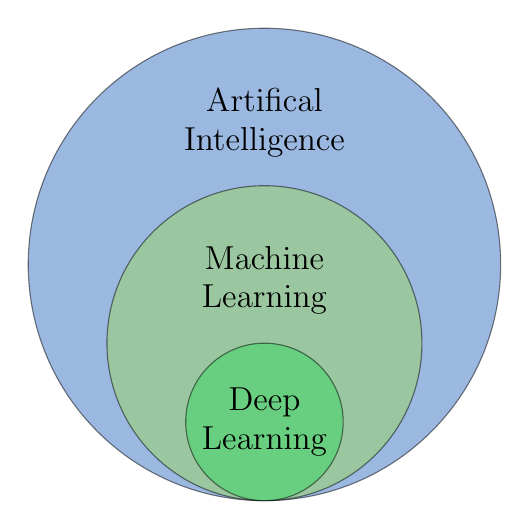
\begin{tikzpicture}
\draw [fill={rgb,255:red,55;green,114;blue,196}, opacity=0.5] (0, 2) circle [radius=3];
\draw [fill={rgb,255:red,155;green,214;blue,96}, opacity=0.5] (0, 1) circle [radius=2];
\draw [fill={rgb,255:red,55;green,214;blue,96}, opacity=0.5] (0, 0) circle [radius=1];
\node [node font=\large, align=center] at (0, 3.8) {Artifical\\ Intelligence};
\node [node font=\large, align=center] at (0, 1.8) {Machine\\ Learning};
\node [node font=\large, align=center] at (0, 0) {Deep\\ Learning};
\end{tikzpicture}
        \end{column}
        \begin{column}{0.5\textwidth}
            \begin{itemize}
                \setlength\itemsep{1em}
                \item [AI:] Az emberi gondolkodás és viselkedés megvalósítása
                      \begin{itemize}
                          \item Intelligens ágensek
                          \item Asimov, Lem, ...
                      \end{itemize}
                \item [ML:] Statisztikai módszerek segítségével tanuló algoritmusok
                      \begin{itemize}
                          \item Felügyelt tanulás
                          \item Felügyelet nélküli tanulás
                          \item Megerősítéses tanulás
                      \end{itemize}
                \item [DL:] Adatok struktúrájának önálló felismerése
                      \begin{itemize}
                          \item Neurális hálózatok
                      \end{itemize}
            \end{itemize}
        \end{column}
    \end{columns}
\end{frame}

\begin{frame}{Néhány ML példa}
    \begin{figure}
        \centering
        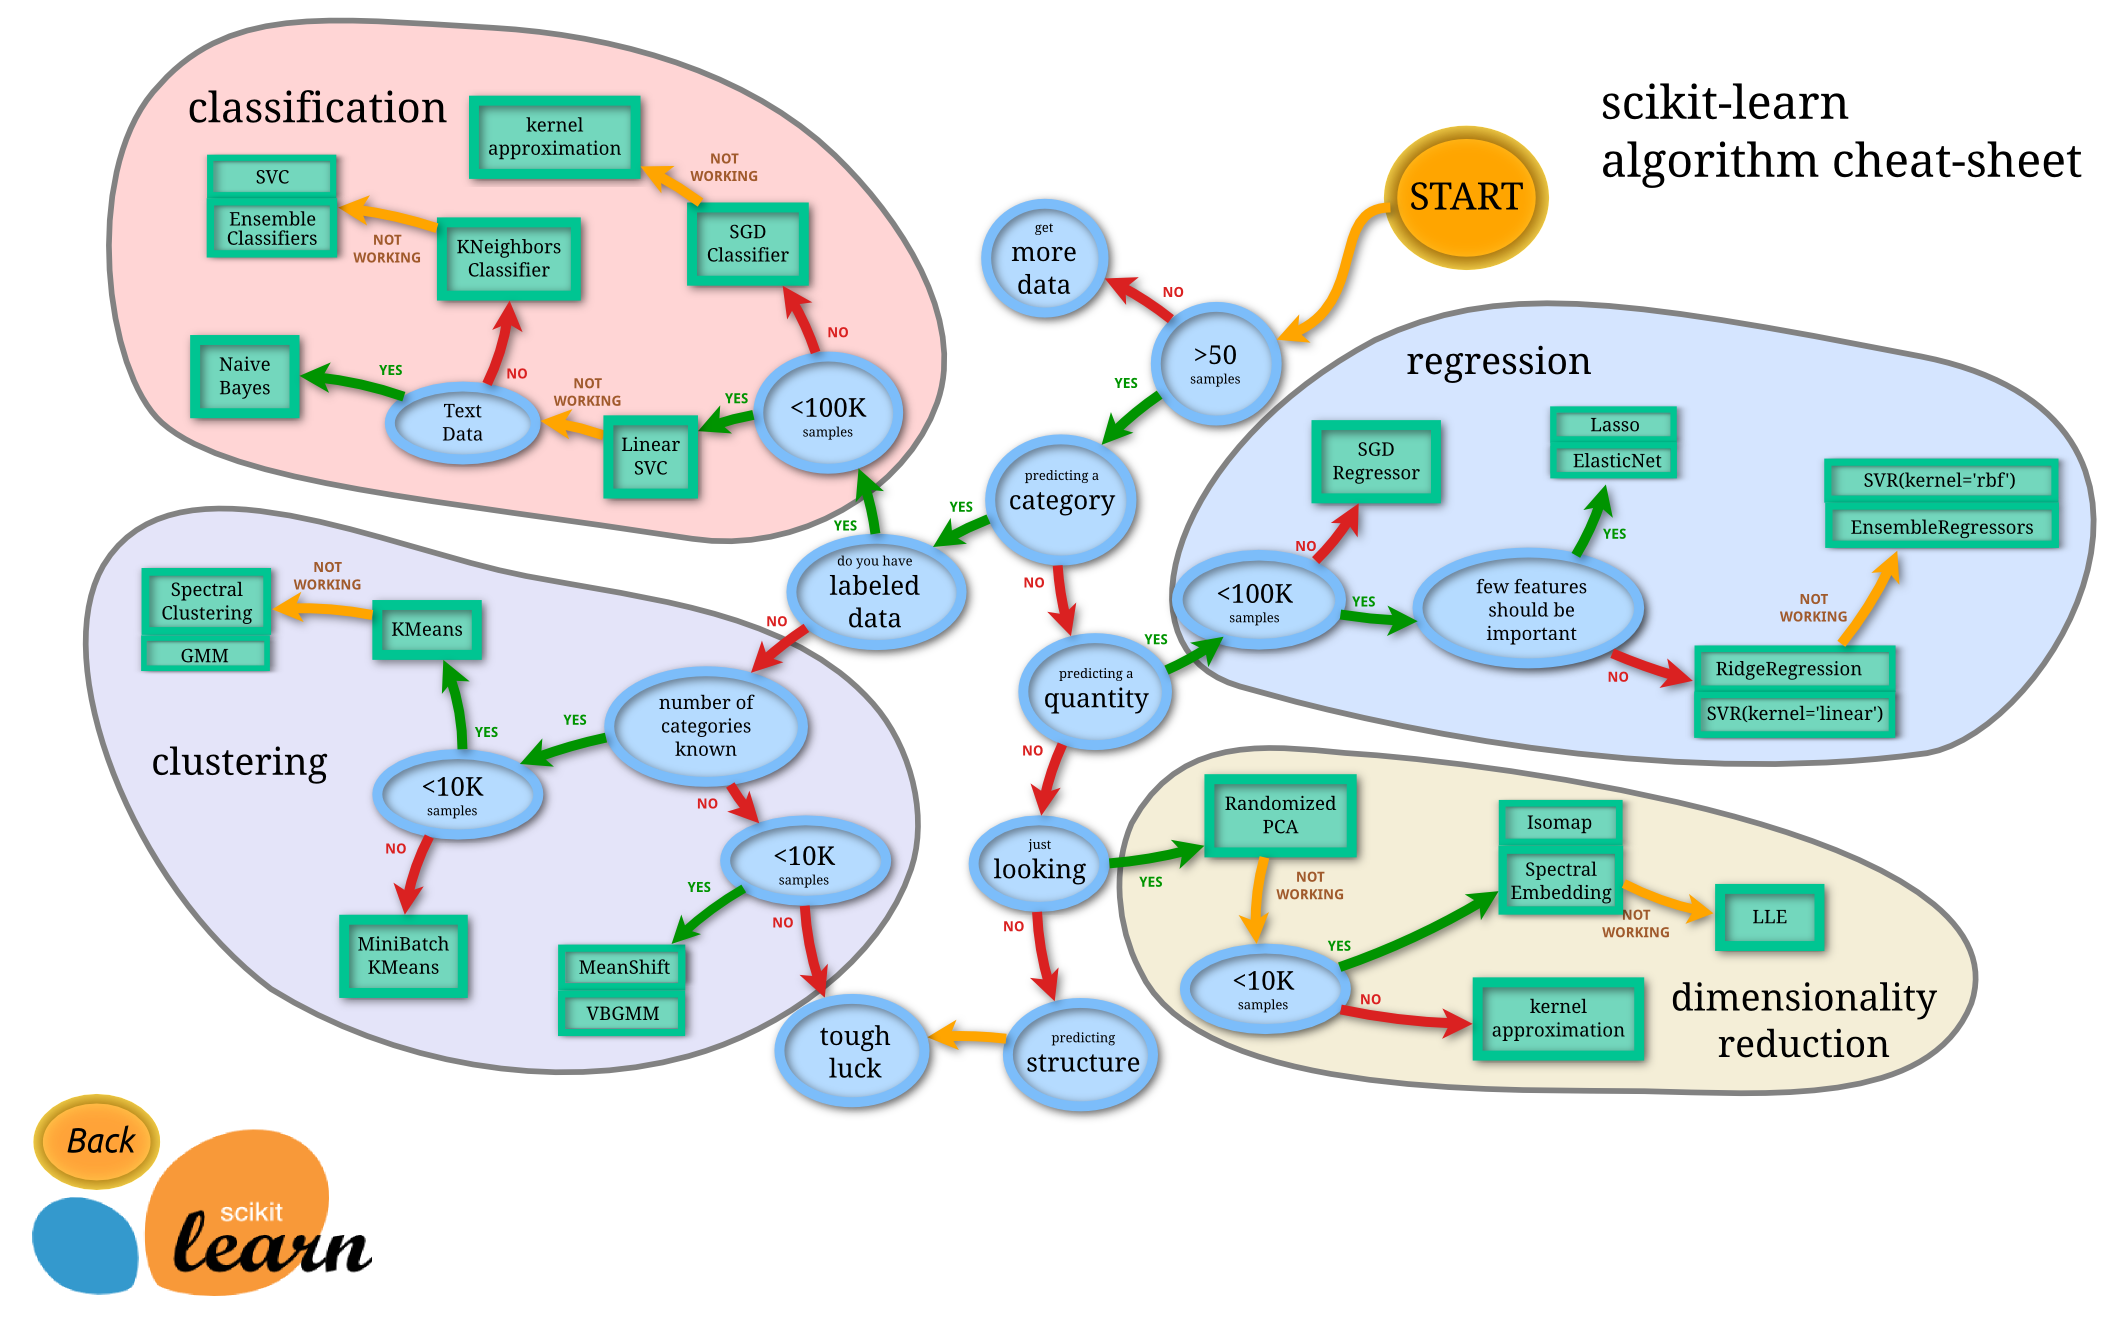
\includegraphics[height=0.7\textheight]{./tex_images/ml_map.png}
        \caption*{Gépi tanulási algoritmusok\footnotemark}
    \end{figure}

    \begin{textblock}{3}(0, 3)
        \tiny
        \begin{itemize}
            \item Elérem-e a csatlakozást?
            \item Jelzéskép felismerés
            \item Található-e pályahiba adott szakaszon?
        \end{itemize}
    \end{textblock}

    \begin{textblock}{3}(0.5, 8)
        \tiny
        \begin{itemize}
            \item Utasok szegmentálása
            \item Járműterhelés osztályozása
            \item Pályaállapot osztályozás
        \end{itemize}
    \end{textblock}

    \begin{textblock}{3}(12.5, 5.5)
        \tiny
        \begin{itemize}
            \item Vonatjegy árazás
            \item Üzemanyagfogyasztás
            \item Pályakarbantartási költségek
        \end{itemize}
    \end{textblock}

    \begin{textblock}{3}(12, 10)
        \tiny
        \begin{itemize}
            \item Fontos paraméterek kiemelése
            \item Számítási kapacitás csökkentése
        \end{itemize}
    \end{textblock}

    \footnotetext{\href{https://scikit-learn.org/stable/tutorial/machine_learning_map/index.html}
        {https://scikit-learn.org/stable/tutorial/machine\_learning\_map/index.html}}
\end{frame}

\begin{frame}{Neurális hálózatok}
    \begin{columns}[b]
        \begin{column}{0.48\textwidth}
            \begin{figure}
                \centering
                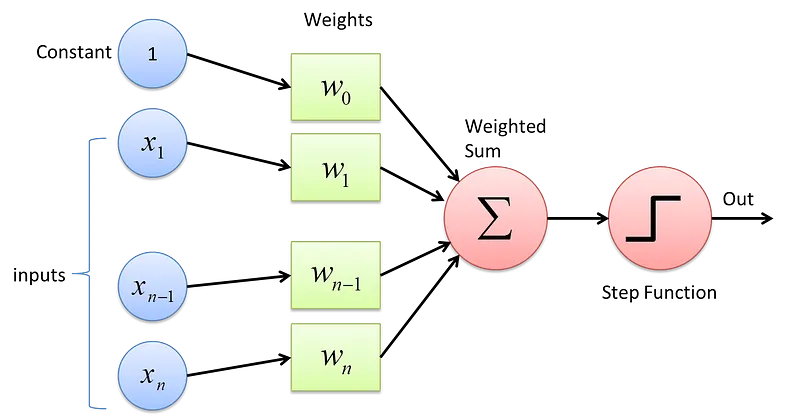
\includegraphics[width=\textwidth]{./tex_images/perceptron.png}
                \caption*{Perceptron\footnotemark[1]}
            \end{figure}
        \end{column}
        \begin{column}{0.48\textwidth}
            \begin{figure}
                \centering
                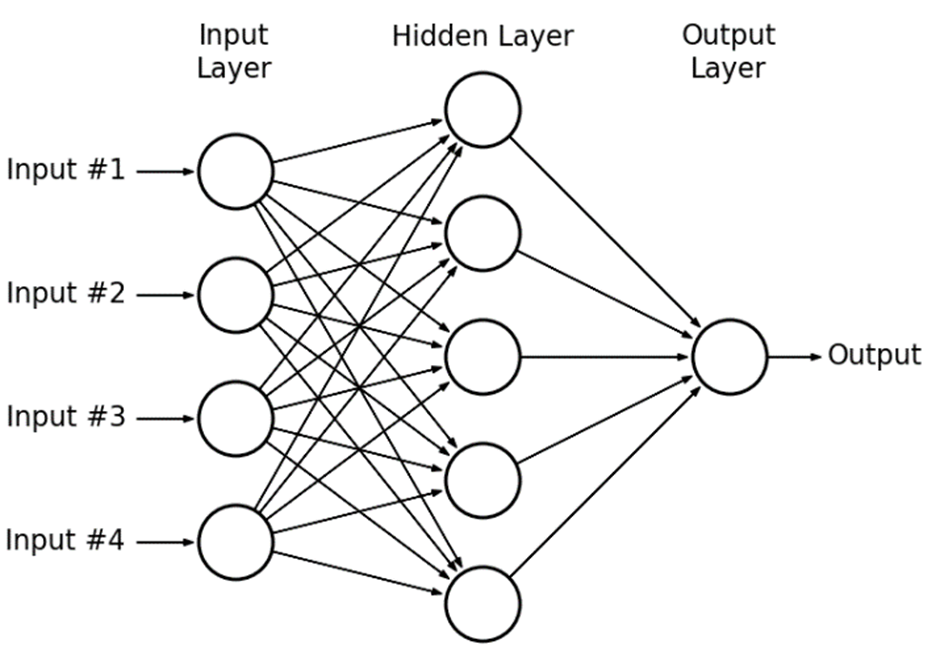
\includegraphics[width=\textwidth]{./tex_images/multi_perceptron.png}
                \caption*{Multilayer Perceptron\footnotemark[1]}
            \end{figure}
        \end{column}
    \end{columns}
    \footnotetext{Source: \href{https://wikidocs.net/165345}{https://wikidocs.net/165345}}
\end{frame}

\begin{frame}{Konvolúciós hálózatok}
    \begin{figure}
        \centering
        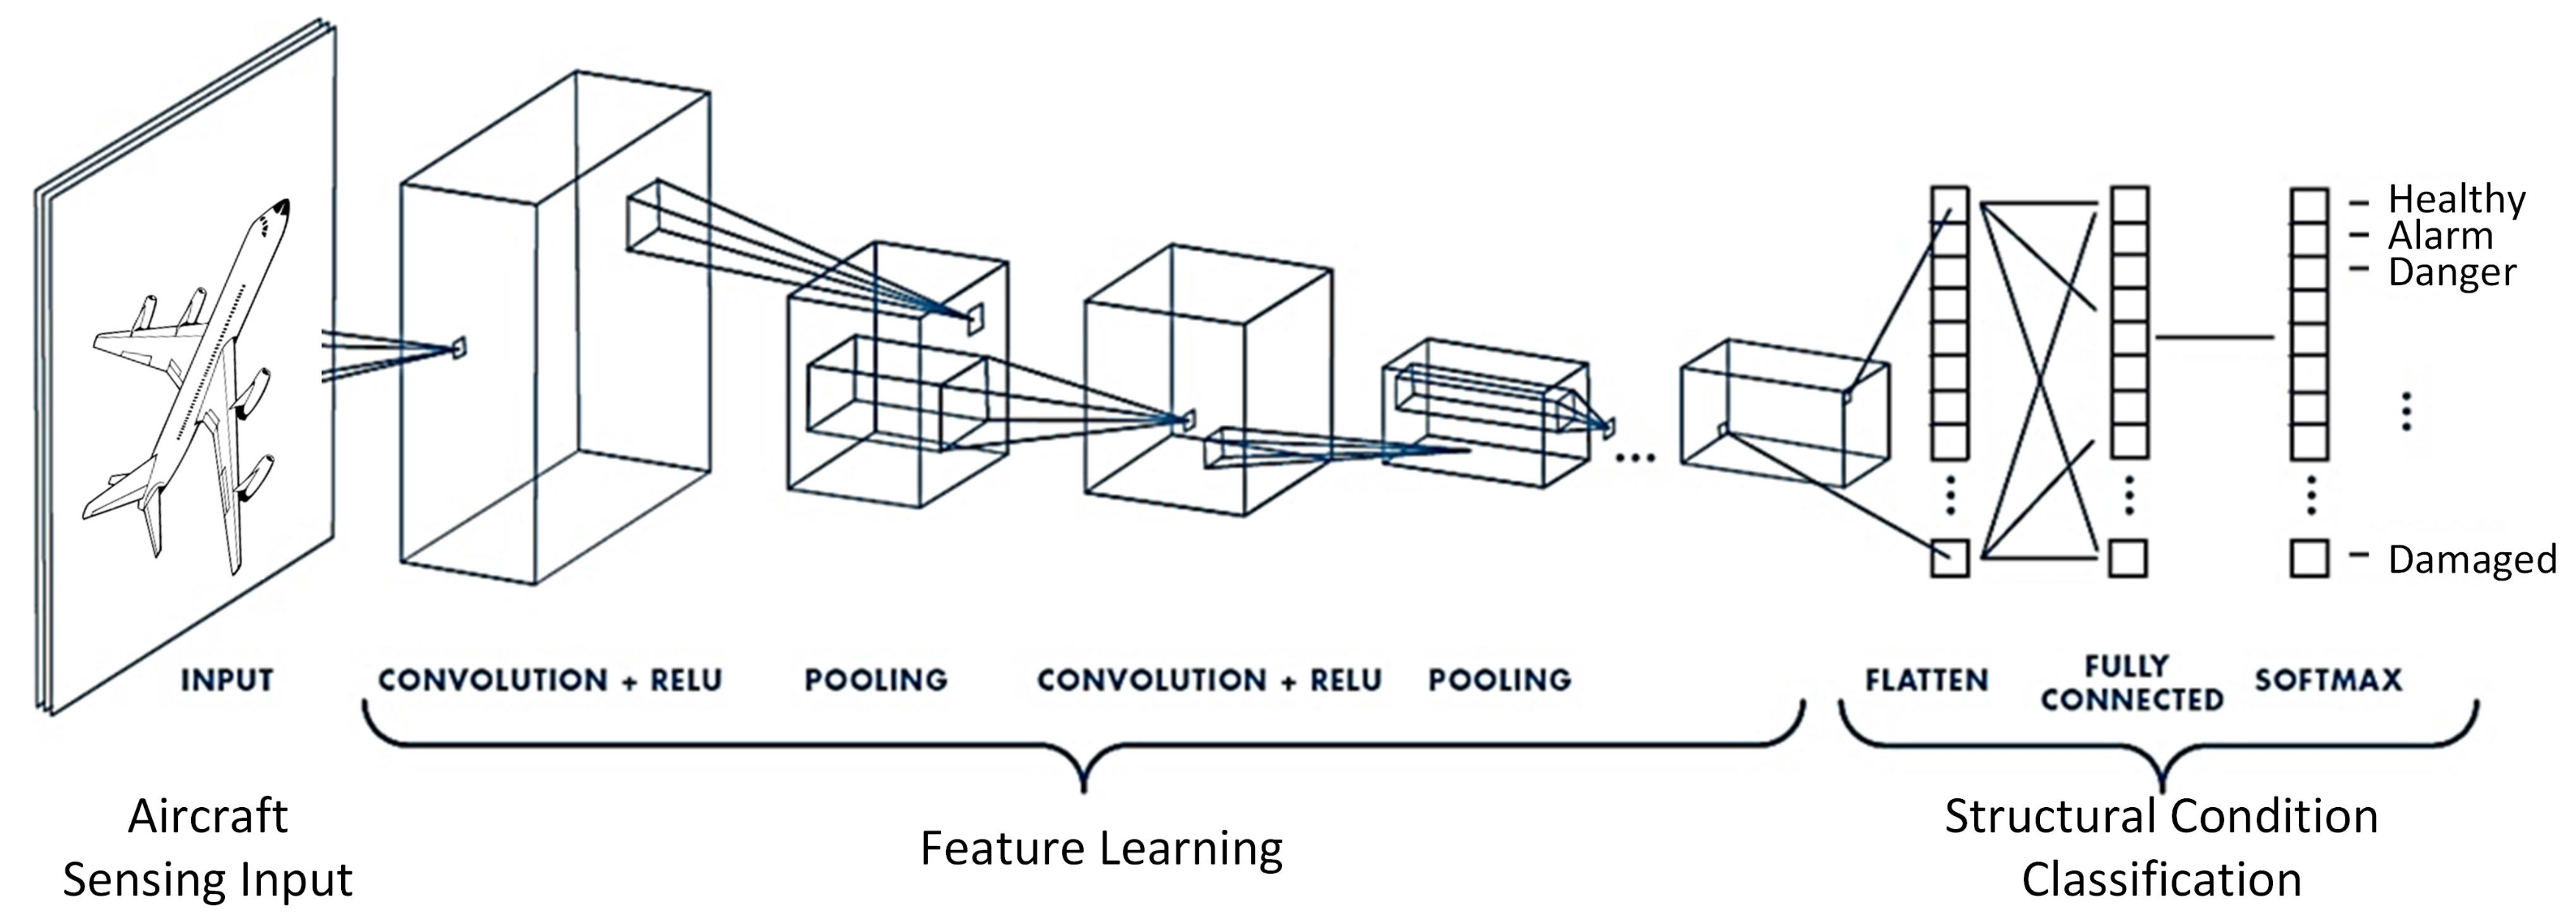
\includegraphics[width=0.9\textwidth]{./tex_images/cnn.png}
        \caption*{Convolutional Neural Network\footnotemark}
    \end{figure}

    \footnotetext{\href{https://wikidocs.net/165345}{https://wikidocs.net/165345}, \href{https://poloclub.github.io/cnn-explainer/}{https://poloclub.github.io/cnn-explainer/}}
\end{frame}

\begin{frame}{Autoencoder}
    \begin{figure}
        \centering
        \begin{subfigure}{0.2\textwidth}
            \centering
            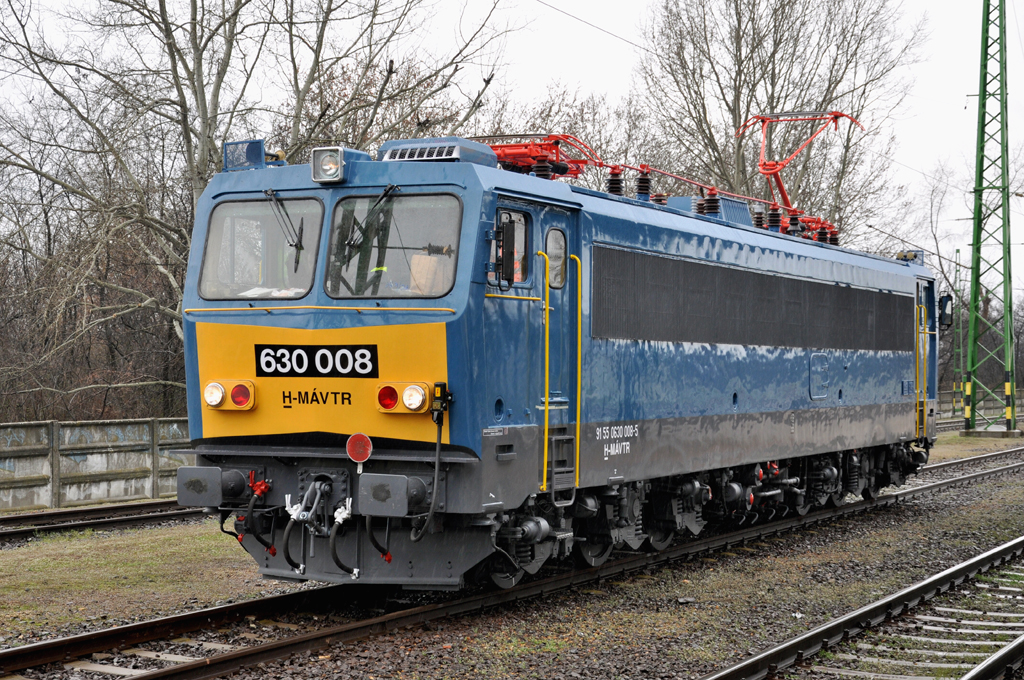
\includegraphics[width=\textwidth]{./tex_images/gigant_2.jpg}
        \end{subfigure}
        \begin{subfigure}{0.4\textwidth}
            \centering
            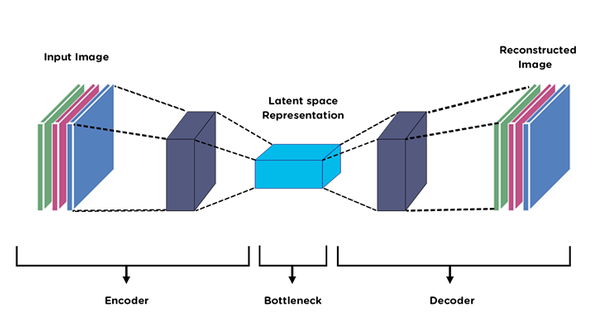
\includegraphics[width=\textwidth]{./tex_images/autoencoder.png}
        \end{subfigure}
        \begin{subfigure}{0.2\textwidth}
            \centering
            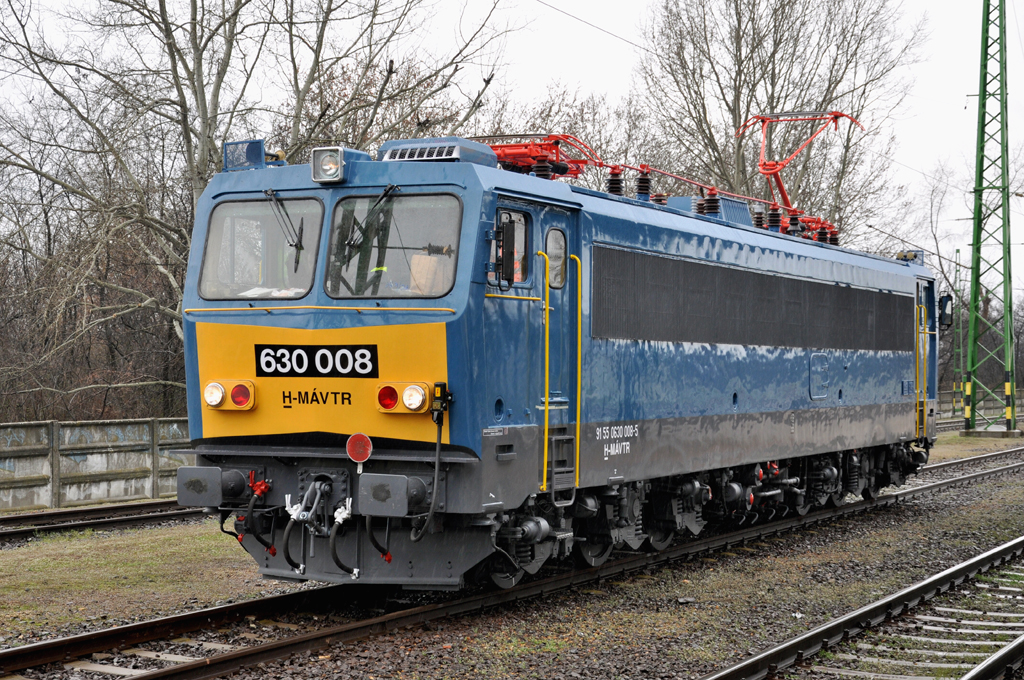
\includegraphics[width=\textwidth]{./tex_images/gigant_2.jpg}
        \end{subfigure}
        \caption*{Autoencoder\footnotemark}
    \end{figure}
    \begin{itemize}
        \setlength{\itemindent}{4em}
        \item [Encoder:] Önállóan meghatározza a leíró paramétereket (Feature Extraction)
        \item [Bottleneck:] Leíró vektorok tere
        \item [Decoder:] Képet generál a vektortér egy eleméből
    \end{itemize}
    \footnotetext{\href{https://wikidocs.net/165345}{https://wikidocs.net/165345},
        \href{https://iho.hu/hirek/eledezik-a-nyolcas-gigant-130321}{https://iho.hu/hirek/eledezik-a-nyolcas-gigant-130321}}
\end{frame}

\begin{frame}{Anomália keresés}

\end{frame}

\begin{frame}
    \centering \Large
    Köszönöm megtisztelő figyelmüket!
\end{frame}

\end{document}